\documentclass[a4paper, 12pt]{article}
%pack{{{
\usepackage[utf8]{inputenc}
\usepackage[russian]{babel}
\usepackage{pdfpages}
\usepackage{graphicx}
\usepackage{float}
\usepackage{listings}
\usepackage{hyperref}
\usepackage{tabularx}
%}}}

%{{{ SETUP

\hypersetup{
	pdfborder={0 0 0}
}

\newcommand{\ra}{\rightarrow}
\newcolumntype{m}[1]{>{$}#1<{$}}
\newcolumntype{t}[1]{>{\tt}#1<{}}

%}}}

\begin{document}

%{{{ ---------- SECTION:Введение ---------
\section{Введение}

Полное наименование программного продукта: <<Интерпретатор коммандной оболочки для встраиваемых систем на базе 
микросхем семейства AVR>>. Продукт создается в рамках курсовой работы по дисциплине ``проектирование трансляторов''.
%}}}

%{{{ ---------- SECTION:Назначение и область применения  ---------
\section{Назначение и область применения}

Система предназначена для записи на микросхемы и последующего использования
для ускорения разработки и отладки аппаратной части встраиваемой системы, создания 
единого протокола обмена данными между микроконтроллером и терминальным управляющим
устройством.
%}}}

%{{{ ---------- SECTION:Технические характеристики  ---------
\section{Технические характеристики}

%{{{ ---------- SUBSECTION: Постановка задачи, применяемые алгоритмы и математические методы ---------
\subsection{Постановка задачи и математические методы} % (fold)
см. \ref{requirements}
%}}}

%{{{ ---------- SUBSECTION: Описание алгоритма функционирования программы ---------
\subsection{Описание алгоритма функционирования программы} % (fold)

Программа осуществляет анализ входных строк, состоящих из ASCII-символов.
\clearpage
Система состоит из следующего набора модулей:
\begin{figure}[H]
	\centering
	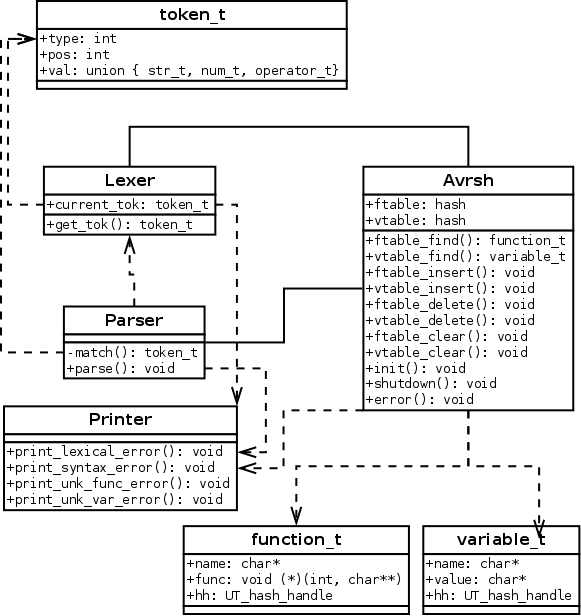
\includegraphics[width=\textwidth]{diag/class.png}
	\caption{Диаграмма классов}
\end{figure}

Модуль {\tt Lexer} осуществляет лексический анализ и токенизацию входной строки. Используя структуру {\tt token\_t} передает данные 
модулю синтаксического анализа. Используется целочисленный тип для передачи типа токена и объединение для передачи значения.

Модуль {\tt Parser} осуществляет синтаксический анализ входной строки.
Представляет собой рекурсивный нисходящий предиктивный распознаватель. Грамматика: см. Приложение \ref{app:grammar}.

Модуль {\tt Avsrh} -- модуль исполнения команд. В нем хранятся 
данные о пользовательских командах, о переменных в виде хеш-таблиц.

Значения переменных хранятся только в виде строк. При необходимости в вычислении-подстановке можно получить числовое значение с помощью оператора {\tt \#\_}. Поддерживаются только целые числа.

Общий алгоритм работы программы:
\begin{figure}[H]
	\centering
	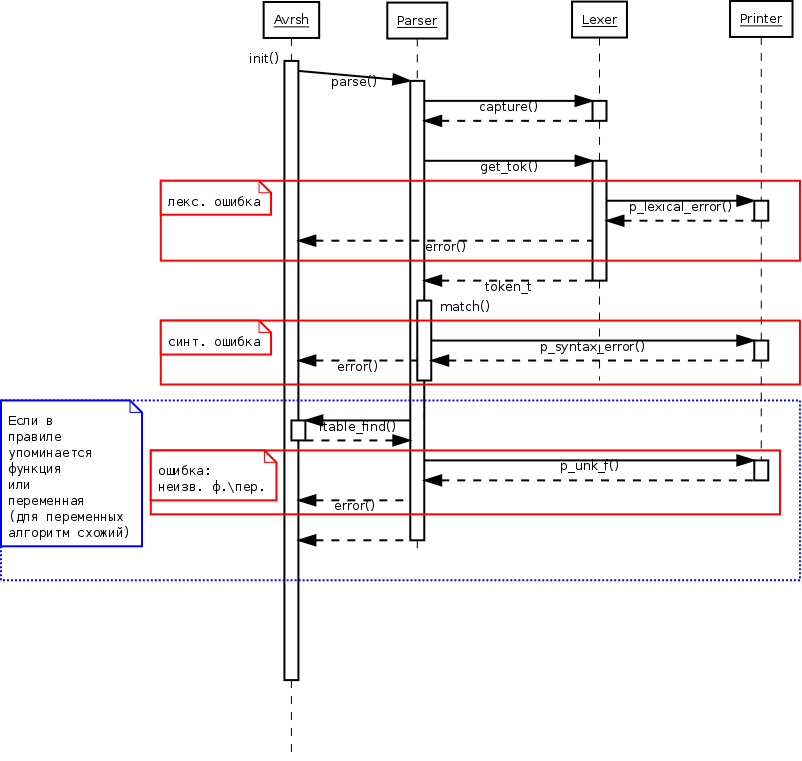
\includegraphics[width=\textwidth]{diag/sequence.png}
	\caption{Диаграмма последовательности}
\end{figure}


%}}}

%{{{ ---------- SUBSECTION: Описание входных и выходных данных ---------
\subsection{Описание входных и выходных данных} % (fold)
%}}}

%}}}

\appendix
\newpage
\addcontentsline{toc}{section}{Приложение}
{\huge Приложение}
%{{{ ---------- SECTION: Исходный код ---------
\section{Приложение А. Грамматика специализированного языка}
\label{app:grammar}

\begin{tabular}{t{r}@{$\hspace{0.5cm}\ra\hspace{0.5cm}$}t{l}}
	control & statement control\\
		& ifst control\\
		& loop control\\
		& set control\\
		& $\epsilon$ \\
	statement 	& ID args DELIM \\
	args		& ID args\\
			& get args\\
			& eval args\\
			& $\epsilon$ \\
	ifst & IF eval branch  \\
	branch & control maybe\_branch  \\
	maybe\_branch & ELSE control END\\
			& ELIF eval branch \\ 
		      & END\\
	loop & WHILE eval control END \\
	set & SET ID \fbox{=} ID\\
	get & \fbox{\$}ID\\
	getn& \fbox{\#}ID \\
	eval & \fbox{(} aexpr \fbox{)}\\
	aexprlv & op \\
	aexprorv& \fbox{+} op \\ 
		& \fbox{-} op \\ 
		& \fbox{*} op \\ 
		& \fbox{/} op \\ 
		& \fbox{\%} op \\ 
		& \fbox{<} op \\ 
		& \fbox{>} op \\ 
		& \fbox{>=} op \\ 
		& \fbox{<=} op \\ 
		& \fbox{==} op \\ 
		& \fbox{!=} op \\ 
		& $\epsilon$\\
	op	& NUMBER \\
		& \fbox{'}ID\fbox{'} \\
		& get\\
		& getn\\
\end{tabular}

%}}}

%{{{ ---------- SECTION: Приложение Б. Грамматика ---------
\section*{Приложение Б. Исходный код}
%}}}


\end{document}
